%!TEX root = ../main.tex
\subsection{Carrier Card Design}
\label{sub:carrier_design}

\subsubsection*{Power Requirements}
\label{sub:power_req}
A carrier card  needs to provide the following voltages for the MicroZed:
\begin{itemize}
	\item $V_{in} = 5V$
	\item $V_{ccio,13}$ (Voltage logic level for I/O bank 13)
	\item $V_{ccio,34}$ (Voltage logic level for I/O bank 34)
	\item $V_{ccio,35}$ (Voltage logic level for I/O bank 35)
\end{itemize}
The different I/0 banks can be operated at different voltage levels.
According to \cite{zynq_dc}, the possibly logic levels for I/O banks are 1.2V, 1.5V, 1.8V, 2.5V, and 3.3V 

It was chosen to supply all I/O banks with a voltage level of 3.3V as there were no need for multiple different levels and 3.3V is widely used.

$$ V_{ccio} =  V_{ccio,13} = V_{ccio,34} = V_{ccio,35} = 3.3V$$

\subsubsection*{Power Up Sequencing}
On power up the first that needs to happen is to pull the MicroZeds PWR\_EN high on the carrier card.
This is done with a pull-up resistor as shown in figure \ref{fig:pwr_en_circuit}.

\begin{figure}
	\centering
	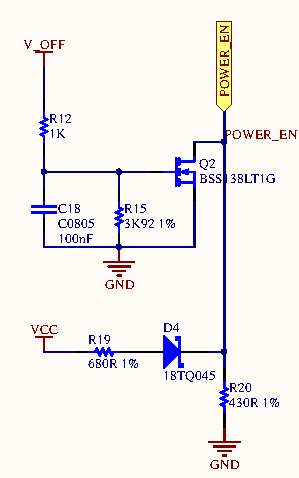
\includegraphics[width=.4\linewidth]{graphics/power_en_sch.pdf}
	\caption{Circuit for proper power sequencing on MicroZeds PWR\_EN.}
	\label{fig:pwr_en_circuit}
\end{figure}

When the MicroZed has powered up its internal DC/DC converters and is ready to receive voltage on its I/O banks the VCCIO\_EN will go high.
VCCIO\_EN has a logic level of 1.8V and the signal is therefore fed to a comparator that outputs a 5V signal to a DC/DC converter when VCCIO\_EN is high.
The DC/DC converter is configured to produce a voltage level of 3.3V that is connected to $V_{ccio}$
This circuitry can be seen in figure \ref{fig:pwr_io_circuit}.

\begin{figure}
	\centering
	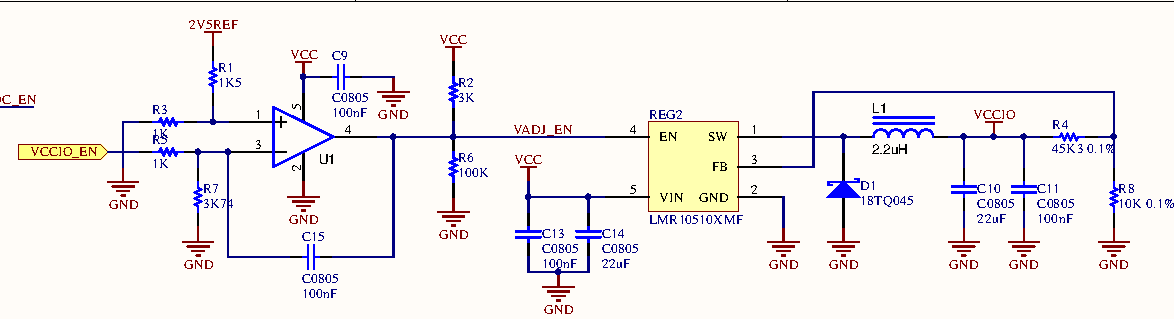
\includegraphics[width=1\linewidth]{graphics/vccio_power_up.pdf}
	\caption{Circuit for proper power sequencing on I/O banks.}
	\label{fig:pwr_io_circuit}
\end{figure}

\subsubsection*{Power Down Sequencing}
On power down VCCIO\_EN, DCDC\_EN and PWR\_EN should be pulled down. 
VCCIO\_EN needs to be pulled down first, hereafter PWR\_EN and lastly DCDC\_EN .
The signals are pulled down by MOSFETS controlled by the V\_OFF signal.
When the power switch on the carrier card is flicked, the battery voltage is connected to the V\_OFF rail thereby turning the MOSFETS on and pulling the signals down. 
The correct sequence is maintained by charging capacitors on the gate side of the MOSFETS thereby creating a delay.
Such a MOSFET circuit is shown in figure \ref{fig:pwr_en_circuit}.


\begin{table}

\centering
\caption{My caption}
\label{my-label}
\begin{tabular}{|p{0.5cm}|p{2cm}|p{1.5cm}|l|l|p{5cm}|}
\hline
\#      & Component              & Quantity & MicroZed Carrier Card & SwarmBot Carrier Card & Comment                                                                                                                                                                                                      \\ \hline
1       & Capacitor              & 7        & 0805ZD226MAT2A        & GRM21BR60J226ME39L    & Found equivalent capacitor as the original comes in packages of 3000.                                                                                                                                        \\ \hline
2       & DNP                    &          &                       &                       &                                                                                                                                                                                                              \\ \hline
3       & Capacitor              & 8        & 06035C104KAT2A        & GCM21BR71H104KA02L    & Found equivalent capacitor with 0805 footprint                                                                                                                                                               \\ \hline
4       & Capacitor              & 4        & 04023C104KAT2A        & C0805C103K5RACTU      & Original was out of stock. Found equivalent capacitor with 0805 footprint                                                                                                                                    \\ \hline
5       & Connector              &          &                       &                       & Equivalent ones will be found at the component storage at SDU                                                                                                                                                \\ \hline
6       & MicroUSB               & 1        & 1981584-1             & 47589-0001            & Original needs to be bought in packs of 10. Found a cheaper equivalent one that can be bought in packs of 5.                                                                                                 \\ \hline
7       & DNP                    &          &                       &                       &                                                                                                                                                                                                              \\ \hline
8       & Schottky Diode         & 1        & MBR230LSFT1G          & SBR2A40P1-7           & Original only ships in packs of 50. Found a a similiar diode with. Has a a higher forward voltage drop, but rough calculations estimate that it will only decrease the efficiency with one percentage point. \\ \hline
9       & Schottky Diode         & 2        & BAT54LT1G             & SBR2A40P1-7           & The SBR2A40P1-7 diode is better in all aspects and 25 of them are already bought for \#8                                                                                                                     \\ \hline
10      & Jumper                 &          & 969102-0000-DA        &                       & Is not needed on the SwarmBot Carrier Card.                                                                                                                                                                  \\ \hline
11      & Connector              &          & 5-146257-3            &                       & Is not needed on the SwarmBot Carrier Card.                                                                                                                                                                  \\ \hline
12      & Bergstak connector     & 2        & 61083-104400LF        & 61083-104400LF        &                                                                                                                                                                                                              \\ \hline
13      & Inductor               & 1        & SRN5020-2R2Y          & SRN5020-2R2Y          &                                                                                                                                                                                                              \\ \hline
14      & DNP                    &          &                       &                       &                                                                                                                                                                                                              \\ \hline
\end{tabular}	
\end{table}

\begin{table}
\centering
\caption{My caption}
\label{my-label}
\begin{tabular}{|p{0.5cm}|p{2cm}|p{1.5cm}|l|l|p{5cm}|}
\hline

15      & MOSFET                 & 2        & BSS138LT1G            & BSS138LT1G            &                                                                                                                                                                                                              \\ \hline
16 - 32 & Resistors              &          &                       &                       & Equivalent ones will be found at the component storage at SDU                                                                                                                                                \\ \hline
33      & Converter              & 1        & LMR10510XMFE/NOPB     & LMR10510XMFE/NOPB     &                                                                                                                                                                                                              \\ \hline
34      & Switch                 & 1        & 1101-M2-S3-C-Q-E-2    &  1101M2S3CQE2         &                                                                                                   \\ \hline
35      & DNP                    &          &                       &                       &                                                                                                                                                                                                              \\ \hline
36      & Comparator             & 1        & AP331AWG-7            & LMV331QDBVRQ1         & Original ships in packs of 50. New comparator is compatible, faster and ships in packs of 5.                                                                                                                 \\ \hline
37      & Programmable reference & 1        & TL431AIDBZR           & TL431AIDBZR           &                                                                                                                                                                                                              \\ \hline
x      & Capacitor for anti-aliasing filter  & 4        & NA           & 08055C102KAT2A           &  Similar to the one used in the MicroZed I/O carrier card and with the 0805 footprint                                                                                                                                                                                                      \\ \hline
x      & Resistors for anti-aliasing fitler  & 8        & NA           &            &  SDUs storage                                                                                                                                                                                                     \\ \hline


\end{tabular}

	
\end{table}
